\chapter{\textbf{Аналитический раздел}}

В данном разделе рассматривается задача анализа существующих алгоритмов классификации.

\section{Постановка задачи}

Классификация документов -- одна из задач информационного поиска, заключающаяся в определении документа к одной из нескольких категорий на основании его содержания. 

Задача распознавания типа удостоверения личности на изображениях, рассматриваемая в данной работе, может быть сформулирована следующим образом. 

Имеется множество документов написанных на естественном языке, и множество заранее известных классов документов. Изображение удостоверения личности Q должно быть отнесено к одному из классов $C=C_i, i \in [0, N]$ с определенной вероятностью.

$C_0$ -- класс прочих изображений, соответствующий значению: <<не является фотографией удостоверения личности, пригодной для идентификации пользователя>>.

\section{Существующие решения}

Необходимо рассмотреть существующие решения и целесообразность создания нового. На рынке представлено множество разнообразных систем, занимающихся распознаванием документов, как платных, так и бесплатных.

\begin{enumerate}
\item[1.] Smart ID Engine \cite{smartengine}.

Все супер, поддерживает международные документы (паспорта, визы, водительские права), отлично распознает, распознает все основные языки, существуют API для различных языков программирования. Работает под различные операционные системы и desktop, и мобильные. 

(очень популярное решение, так как и на русско и н английском это первая ссылка)

Минусы??
Только если платное.

\item[2.] ABBYY \cite{abbyy}.

Только на мобильные устройства.

Паспорта и документы РФ, международные документы.

Платное.

\item[3.] IRIS \cite{iris}.

Только документы США и международные паспорта и ID-карты. 

Платное.

\item[4.] Jumio \cite{jumio}.

Европа и США. Платное.

\item[5.] Idmatch \cite{idmatch}.
\end{enumerate}

Id-карты Кыргызской Республики. Предоставляют API, нет готового ПО.

Бесплатное.

\textbf{Вывод} следует такой, что IRIS, Jumio, Idmatch -- не идентифицируют необходимые документы. ABBYY -- решение только для мобильных устройств. Smart ID Engine -- идеальная система..

\section{Визуальное представление документа}

Далее необходимо рассмотреть этапы обработки изображения, а именно методы классификации по визуальным и текстовым признакам.

Для начала, рассмотрим способы классификации документов по визуальным признакам.

\subsection{Методы классификации}

Существует множество методов классификации, которые используют различный математический аппарат и различные подходы при реализации. Однако эффективность этих методов зависит от конкретной решаемой задачи. Несмотря на то, что последнее десятилетие коммерческие компании занимаются проблемой повышения качества машинного обучения, на сегодняшний день не существует методов, которые могли бы однозначно эффективно решить задачу классификации. 

Можно выделить следующие типы методов классификации: вероятностные, метрические, логические, линейные, логическая регрессия. Обобщенно опишем некоторые из них, указывая преимущества и недостатки каждого из них. 

\begin{enumerate}
\item[1.] Метод Байеса.

Метод Байеса (Naive Bayes, NB) относится к вероятностным методам классификации \cite{baes}. 

Пусть имеется множество классов $C = \{c_0, c_1, ..., c_N\}$ документов. Согласно теореме Байеса вероятность того, что документ принадлежит классу $c$, имеет вид \ref{eq:baies}.

\begin{equation}
	\centering
	P(c|d)=\frac{P(c)P(d|c)}{P(d)}
	\label{eq:baies}
\end{equation}

Вероятность $P(d)$ не требует вычислений ввиду того, что его значение не зависит от класса $c$, а значит, не влияет на нахождение наибольшей вероятности. 

Преимущества метода состоит в следующем: 
\begin{itemize}
\item высокая скорость работы;
\item поддержка инкрементного обучения;
\item простая реализация алгоритма в виде программы,;
\item легкая интерпретируемость результатов работы алгоритма. 
\end{itemize}

Несмотря на приведенные достоинства, метод Байеса имеет так же и минусы в своей реализации. 
\begin{itemize}
\item Относительно низкое качество классификации. 
\item Неспособность учитывать зависимость результата классификации от сочетания признаков являются главными недостатками этого метода.
\end{itemize}

\item[2.] Метод k ближайших соседей.

Метод k ближайших соседей (k Nearest Neighbors, KNN) относится к метрическим методам и считается простейшим классификатором \cite{neighbors}. Суть метода заключается в том, что документу $d$ присваивается тот класс $c$, к которому принадлежит большинство из $k$ ближайших соседей документа, вычисленных с помощью какой-либо метрики расстояния.

Достоинства данного метода: 
\begin{itemize}
\item простая реализация;
\item проработанная теоретическая база;
\item адаптация под нужную задачу выбором метрики;
\item интерпретируемость.
\end{itemize}

К недостаткам относятся: 
\begin{itemize}
\item недостаточная производительность в реальных задачах, так как число соседей, используемых для классификации, будет достаточно большим; 
\item трудность в наборе подходящих весов и определением, какие признаки необходимы для классификации; 
\item зависимость от выбранной метрики расстояния между примерами.
\end{itemize}

\item[3.] Метод деревьев решений.

Метод деревьев решений (Decision Trees, DT) относится к логическим методам классификации \cite{tree}. Дерево решений представляет собой конечный связный граф с множеством вершин, по которому производится классификация документов, описанных набором признаков. В узлах (вершинах) дерева прописаны условия, после проверки которых выполнение алгоритма классификации продолжается по правому или левому поддереву рассматриваемого узла. Процедура повторяется в каждом посещенном узле до тех пор, пока очередной узел не окажется листом. У каждого узла столько ветвлений, сколько значений имеет выбранный признак. 

Метод обладает рядом преимуществ, таких как:
\begin{itemize}
\item простота восприятия алгоритма;
\item быстрота обучения;
\item высокая точность прогнозирования. 
\end{itemize}

Однако также присущи и недостатки, такие как:
\begin{itemize}
\item неустойчивость алгоритмов к выбросам;
\item с увеличением размера обучающего множества увеличение затрачиваемого на построение дерева времени.
\end{itemize}

\item[4.] Метод опорных векторов.

Метод опорных векторов (Support Vector Machine, SVM) является линейным методом классификации, в настоящее время призван одним из лучших \cite{vectors}. Главным принципом SVM является определение раз- делителя в искомом пространстве, который разделяет классы наилучшим образом.

Одно из преимуществ SVM-метода в том, что так как он пытается определить оптимальное направление разделения признакового пространства, рассматривая комбинации признаков, он достаточно устойчив к большим размерностям. 

Потенциальные недостатки метода опорных векторов заключается в следующем: невозможность калибровки вероятности попадания в определенный класс, подходит только для решения задач с 2 классами, параметры модели сложно интерпретировать.

\item[5.] Линейный метод наименьших квадратов.

Одним из ранних применений регрессии к классификации текстов является линейный метод наименьших квадратов (ЛМНК) \cite{linear}.

Как и в случае случае классификатора SVM, обучение регрессионной модели так же использует затратный оптимизационный процесс

Линейный метод наименьших квадратов показал себя устойчивым на практике.

\item[6.] Нейронные сети.
\end{enumerate}

Нейронные сети состоят из набора <<нейронов>>, которые являются преобразователями входных сигналов в выходные \cite{neuron}. Преобразование задается весами сети, которые являются параметрами и могут изменяться. Выходные сигналы вычисляются как функция от входных сигналов. В общем случае нейронная сеть строится как соединение множества нейронов, объединенных в уровни, при этом выходы одного уровня являются входами следующего.
Самая простая нейронная сеть состоит из одного слоя, однако круг решаемых такими сетями задач ограничен. Поэтому на практике часто используют нейронные сети, содержащие большее число слоев.

Преимуществом нейронных сетей является их способность аппроксимировать любую непрерывную функцию. 

Однако, как показали многочисленные исследования, нейронные сети не лишены и недостатков. Существенным недостатком нейронных сетей является то, что результат классификации полностью зависит от начальных установок сети. Поэтому качество обучения сети тем выше, чем больше тестовых примеров участвует в обучении. 

Оптимальным методом классификации являются \textbf{нейронные сети}. 

Существует множество архитектур нейронных сетей, необходимо проанализировать и сравнить их.

\subsection{Выбор архитектуры нейронной сети.}

Задача классификации изображений является популярной и хорошо изученной. Выбор алгоритма классификации будет производится на базе результатов международного соревнования ILSVRC \cite{ILSVRC} (ImageNet Large Scale Visual Recognition Challenge). Соревнование оценивает алгоритмы обнаружения объектов и классификации изображений. Его целью является выявление самых лучших с точки зрения точности и скорости алгоритмов обнаружения и классификации. Оценка алгоритмов производится с помощью выборки данных ImageNet \cite{imagenet}. Эта выборка представляет из себя большую визуальную базу данных, содержащую более 14 миллионов изображений, которые в свою очередь разбиваются на 21841 категорию.

Начиная с 2012 года данное соревнованию выигрывают сверточные нейронные сети (Convolutional Neural Networks), а именно AlexNet \cite{alexnet}, ZFNet \cite{zfnet}, VGGNet \cite{vggnet}, GoogLeNet \cite{googlenet}, ResNet \cite{resnet}, TrimpsNet (Не было никакого нового научного вклада, который оправдывал бы подготовку статьи, и по этой причине авторы TrimpsNet только поделились результатами) и SENet \cite{senet}. С 2015 года CNN превзошли человеческие показатели -- 5.1\% \cite{human}. 

\begin{enumerate}
\item[1.] Архитектура AlexNet.

AlexNet была первой свёрточной нейросетью, выигравшей соревнование по классификации ImageNet в 2012 году. Архитектура AlexNet состоит из пяти свёрточных слоёв, между которыми располагаются pooling-слои и слои нормализации, а завершают нейросеть три полносвязных слоя.

На схеме архитектуры все выходные изображения делятся на два одинаковых участка -- это связано с тем, что нейросеть обучалась на старых GPU GTX580, у которых было всего 3 ГБ видеопамяти. Для обработки использовались две видеокарты, чтобы параллельно выполнять операции над двумя частями изображения.

\item[2.] Архитектура ZFnet.

В 2013 году нейросеть ZFnet смогла достичь результата 11.7\% -- архитектура AlexNet использовалась в качестве основы, но с изменёнными параметрами и слоями. 

\item[3.] Архитектура VGGnet.

Появилась в 2014 году. Основная идея -- использовать вместо больших сверток (11x11 и 5x5) маленькие свертки (3x3). С маленькими фильтрами мы получим не так много параметров, но при этом сможем гораздо эффективнее обрабатывать их.

\item[4.] Архитектура GoogleNet.

GoogleNet или Inception-v1 -- ещё более глубокая архитектура с 22 слоями. Целью Google было разработать нейросеть с наибольшей вычислительной эффективностью. Для этого они придумали так называемый модуль Inception --- вся архитектура состоит из множества модулей, следующих друг за другом.

\item[5.] Архитектура ResNet.

ResNet -- это сокращенное название для Residual Network (дословно  -- «остаточная сеть»). Решает проблему деградации (простая сеть увеличивает частоту ошибок по мере того, как сеть углубляется), и после использования остатка, когда сеть углубляется, частота ошибок все еще может уменьшаться.

\item[6.] Архитектура SENet.

Squeeze-and-Excitation Networks (SENets) представляют собой специальный блок для свёрточной нейронной сети, который улучшает взаимозависимости каналов практически без дополнительных вычислений. Основная идея -- добавить параметры к каждому каналу свёрточного блока, чтобы сеть могла адаптивно регулировать вес каждой карты признаков. 

\end{enumerate}

Результаты сравнения архитектур представлены в таблице \ref{table:cnncompare}.

\begin{table}[H]
\caption{Сравнение архитектур сверточных нейронных сетей. }
\begin{tabular}{|p{2.5cm}|p{1.5cm}|p{2cm}|p{5cm}|p{4cm}|}
\hline
Название сети \cite{cnn} & Год & Ошибка Top-5 & Количество обучаемых параметров \cite{numparams} & Требуемое оборудование \cite{gpu} \\ \hline
AlexNet       & 2012 & 16.4 \%  & 60 миллионов  & 2 GPU \\ \hline
ZFNet         & 2013 & 11.7 \%   & 60 миллионов   & 1 GPU \\ \hline
VGGNet        & 2014 & 7.3 \%    & 138 миллионов  & 4 GPU \\ \hline
GoogleNet     & 2014 & 6.7 \%    & 4 миллиона & CPU \\ \hline
ResNet        & 2015 & 3.5 \%    & 25.6 или 1.7 миллиона  & 2 GPU \\ \hline
TrimpsNet     & 2016 & 2.99 \%   &  & \\ \hline
SENet         & 2017 & 2.25 \%   & 27.5 миллионов  & 8 GPU \\ \hline
\end{tabular}
\label{table:cnncompare}
\end{table}

В соответствии с результатами ILSVRC последних лет, можно отметить, что наилучшей точностью классификации объектов на сегодняшний день обладает свёрточная нейронная сеть SENet. Однако этот алгоритм является очень требовательным к вычислительным ресурсам.

Принято компромиссное решение -- использовать архитектуру нейронной сети GoogleNet, так как она дает хорошие показатели точности и не требует мощные вычислительные ресурсы.

\section{Обзор и анализ методов распознавания и классификации текстовой информации}

Второй составляющей метода является распознавание и классификация текстовой информации в документе.

Выше уже были рассмотрены методы классификации.

Таким образом, процесс делится на два связанных между собой этапа:

\begin{itemize}
\item этап преобразования изображения в вектор признаков, в процессе которого определяется наиболее полное и информативное представление изображения в виде числового вектора;
\item этап классификации, в процессе которого проверяется гипотеза принадлежности изображения классу изображений объекта на основании наблюдения (вектор признаков).
\end{itemize}

\subsection{Оптическое распознавание символов}

Преобразованием графического изображения в текст занимаются специальные программы распознавания текста (Optical Character Recognition - OCR).

Основной принцип автоматического распознавания образов -- это обучение машины определению всевозможных эталонных образцов, с
которыми будет сравниваться распознаваемый объект. В OCR-системах это буквы, цифры, знаки препинания. Обучение осуществляется за счет того, что машине показываются образцы символов различных классов. На основании этих образцов машина формирует прототип описания каждого
класса объектов. Затем в процессе распознавания неизвестные символы сравниваются с заранее полученными образцами и определяется класс, с
которым обнаружено больше всего совпадений.

Системы оптического распознавания текста -- OCR-системы (optical character recognition) технология, которая позволяет преобразовывать различные типы документов, такие как отсканированные документы, PDF-файлы или фото с цифровой камеры, в редактируемые форматы с возможностью поиска \cite{ocr}. 

OCR -- это одно из направлений компьютерного зрения. 

Современные системы оптического распознавания можно разделить на коммерческие и свободно распространяемые системы с открытыми исходными кодами.

В контексте задач массовой оцифровки интерес представляют как коммерческие системы по причине высокого качества, так и открытые системы по причине своей доступности и гибкости в настройке. Поскольку целью данной работы является обработка русскоязычных документов, то интерес представляют системы с поддержкой распознавания русского языка.

ABBYY FineReader \cite{finereader} -- это программное обеспечение оптического распознавания символов (OCR). Для распознавания текста поддерживается до 190 языков. OCR или распознавание текста, использует интеллектуальные алгоритмы, которые преобразуют изображения в редактируемый текст, сохраняя исходный макет и форматирование исходного документа. Является признанным лидером на рынке. Распространяется на коммерческой основе.

IRIS Readiris \cite{readiris} -- это программа для преобразования документов в различные форматы. Распознает более 130 языков, включая русский, принимает файлы и сохраняет результаты во всех возможных форматах. Программное обеспечение платное. 

Cuneiform \cite{cuneiform} -- свободно распространяемая открытая система оптического распознавания текстов российской компании Cognitive Technologies. CuneiForm позиционируется как система преобразования электронных копий бумажных документов и графических файлов в редактируемый вид с возможностью сохранения структуры и гарнитуры шрифтов оригинального документа в автоматическом или полуавтоматическом режиме. Система включает в себя две программы для одиночной и пакетной обработки электронных документов. Поддерживает все необходимые нам языки: английский, русский, испанский, итальянский, французский, немецкий. Кроме того, поддерживается смесь русского и английского языка. 

Tesseract \cite{tesseract} -- свободная компьютерная программа для распознавания текстов, разрабатывавшаяся Hewlett-Packard, а затем Google купил её и открыл исходные тексты под лицензией Apache 2.0 для продолжения разработки. Сегодня Tesseract считается одним из самых мощных решений с открытым исходным кодом (open-source) для распознавания данных со сканированных документов. Tesseract поддерживает более 100 различных языков, что делает его универсальным и широко распространённым решением во всём мире. Многие технологические компании используют Tesseract в основе для построения комплексных решений по интеллектуальной обработке данных.

OCRFeeder \cite{ocrfeeder} -- программа, предоставляющая графический интерфейс пользователя для систем оптического распознавания символов CuneiForm, Tesseract, GOCR и Ocrad. OCRFeeder является свободно распространяемой программой для операционной системы Linux.

Выбор OCR систем основывался на сравнительном анализе их результатов по трем типам данных (среднее качество, высокое качество и очень высокое качество) \cite{textocr}. Примеры изображений приведены на рисунках \ref{img:quality1}, \ref{img:quality2}, \ref{img:quality3}.

\begin{figure}[H]
	\centering
	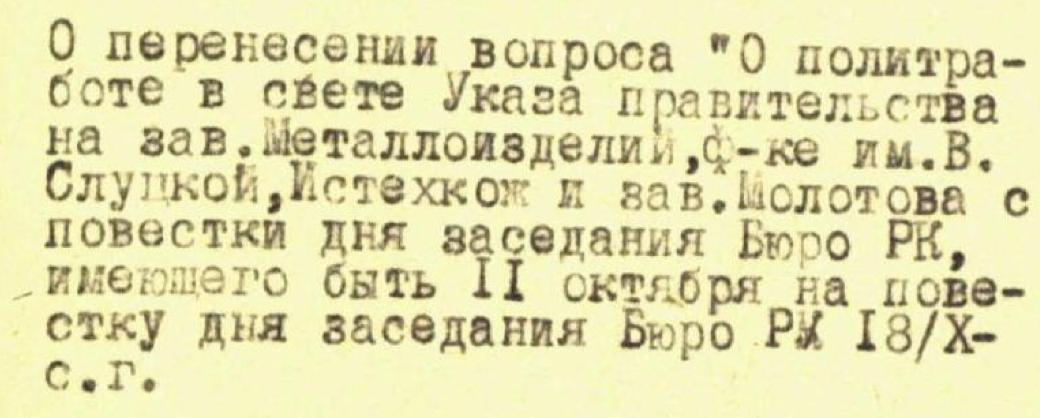
\includegraphics[scale=0.7]{quality1}
	\caption{Среднее качество. }
	\label{img:quality1}
\end{figure}

\begin{figure}[H]
	\centering
	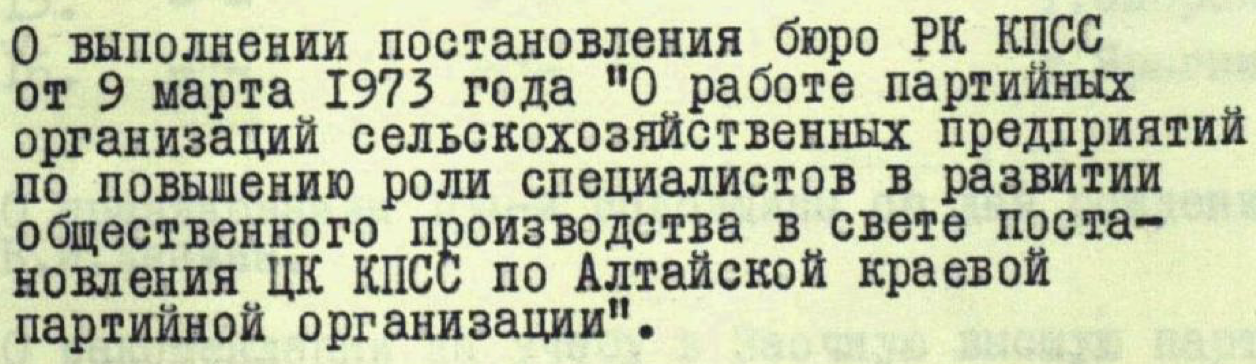
\includegraphics[scale=0.7]{quality2}
	\caption{Высокое качество. }
	\label{img:quality2}
\end{figure}

\begin{figure}[H]
	\centering
	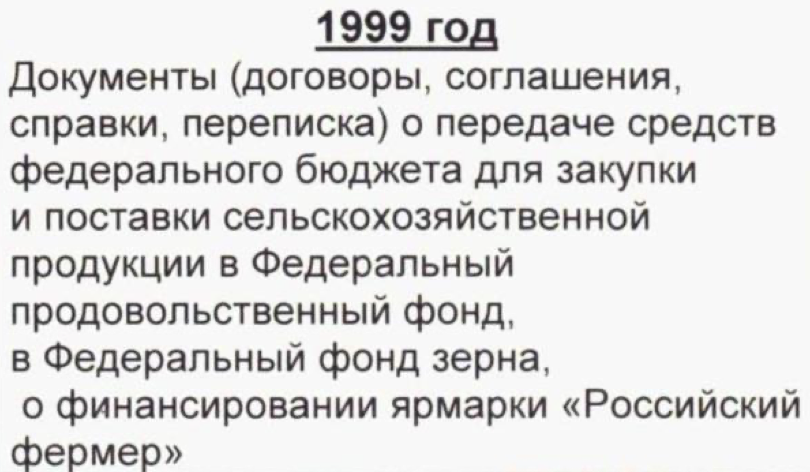
\includegraphics[scale=0.7]{quality3}
	\caption{Очень высокое качество. }
	\label{img:quality3}
\end{figure}

Качество результатов распознавания представлено в таблице \ref{table:comparetext}.

\begin{table}[H]
\caption{Сравнение качества распознавания текста.}
\begin{tabular}{|p{3cm}|p{3cm}|p{3cm}|p{3cm}|p{3cm}|}
\hline
& Качество распознавания документов среднего качества & Качество распознавания документов высокого качества & Качество распознавания документов очень высокого качества & Доступность \\ \hline
ABBYY FineReader & 76,8\% & 90,55\% & 99,25\% & коммерческое\\ \hline
IRIS Readiris & 22,01\% & 68,34\% & 94,40\% & коммерческое \\ \hline
Cuneiform & 0\% & 30,28\% & 90,20\% & бюджетное \\ \hline
Tesseract & 36,06\% & 74,68\% & 94,13\% & бюджетное \\ \hline
\end{tabular}
\label{table:comparetext}
\end{table}

Полученные результаты сравнительного анализа свидетельствуют о том, что коммерческая система <<Abby Finereader>> достигает максимального уровня качества. Среди свободно распространяемых систем наилучшей является Tesseract.

\section{Вывод}

В данном разделе описаны способы визуального сравнения изображений, распознавания и классификации текстовой информации.
